\documentclass[10pt]{exam}
\usepackage[hon]{template-for-exam}
\usepackage{enumitem}
\usepackage{tikz}
\usepackage{multicol,graphicx,cclicenses}
\usetikzlibrary{shadings,decorations.pathmorphing,arrows.meta}



\def\mytitle{Chapter 7 (Momentum)}
\author{Rohrbach}
\date{\today}

\def\mymaketitle{
  \begin{flushleft}
    {\LARGE \textbf \mytitle \par}
  \end{flushleft}
}



\begin{document}


\mymaketitle



\newcommand{\stampbox}[1]{

  \hfill
  \begin{tikzpicture}[every text node part/.style={align=center}]
     \node[gray!50,draw,rounded corners] at (0,0) 
      {\sc Stamp \\ \sc Here \\ \small #1 \sc Points};
  \end{tikzpicture}
  \vspace{1em}
  
  \hrule

}


\begin{center}
  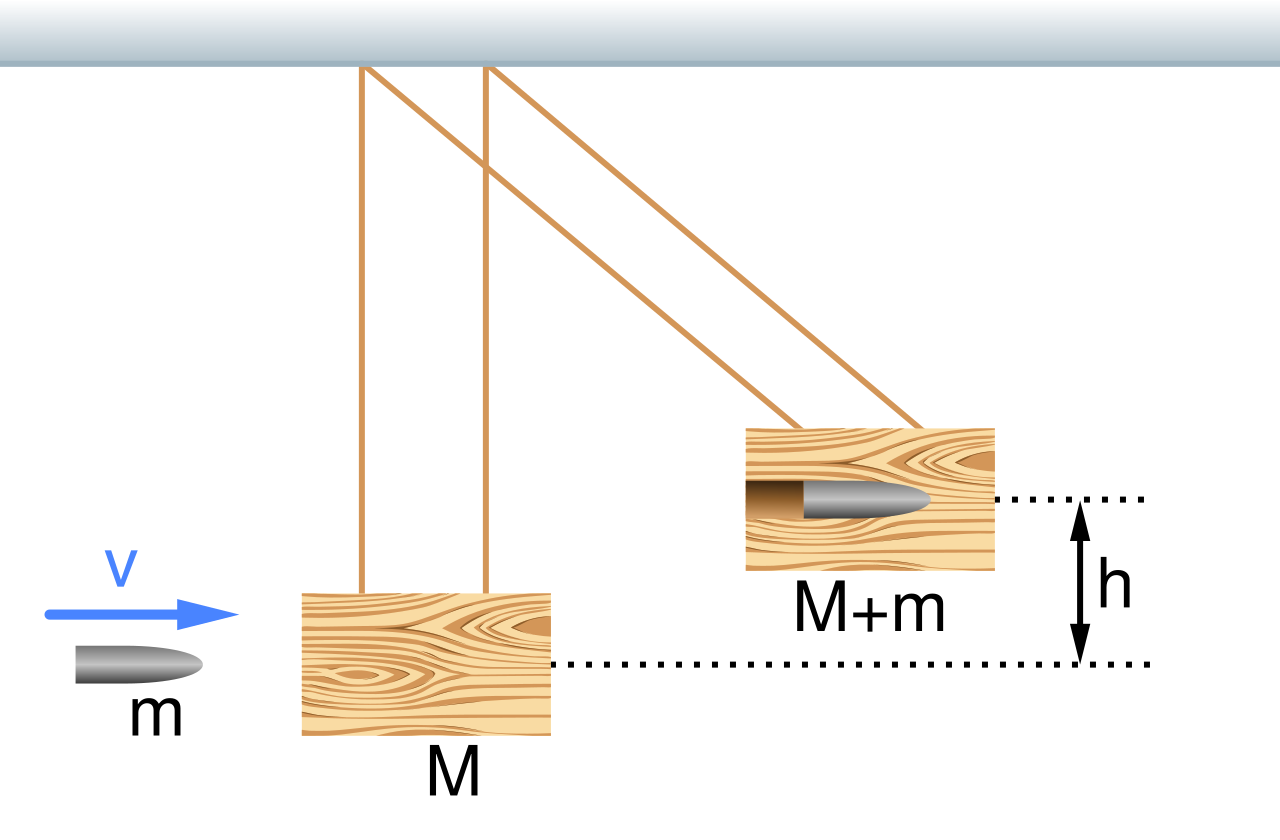
\includegraphics[height=4.1cm]{ballistic-pend.png}
  
  {\small``Sketch of a ballistic pendulum before and after it is struck by a bullet'' by \texttt{MikeRun}} 
  
  \cc\hspace{-1em}\ccby\hspace{-.7em}\ccsa  {\small CC BY-SA 4.0}
  
\end{center}


%%%%%%%%%%%


\section*{Homework Check A (collected Thu, Jan 15)}


%%%%%%%%%%%


\paragraph{Momentum and its Conservation} p. 192 \#1, 2, 3, 5, 6, 7, 9, 11
\dotfill Complete by Mon, Jan 13

\stampbox{5}

%%%%%%%%%%%


\paragraph{Collisions and Impulse} p. 192 \#15, 16, 18
\dotfill Complete by Mon, Jan 13

\stampbox{5}


%%%%%%%%%%%


\paragraph{Elastic Collisions} pp. 193 \#25, 26, 27, 30, 71
\dotfill Complete by Thu, Jan 15

\hfill \textbf{\emph{Homework Quiz}}

\stampbox{5}


%%%%%%%%%%%






\subsection*{Answers}

\begin{multicols}{3}

  \begin{itemize}[noitemsep]
    \item[1.] 0.235 kg m/s
    \item[2.]  5.8 m/s
    \item[3.]   10.2 m/s
    \item[5.]  \SI{5.85e7}{\newton}
    \item[6.]  13,860 kg
    \item[7.]  0.90 m/s
    \item[9.]  2,500 m/s
    \item[11.]  0.99 m/s
    \item[15.]  2233 N
    \item[16.]  (a) 1.71 N s; (b) 489 N
    \item[18.]  2.38 N s to the left
    \item[25.]  1.27 m/s;   5.07 ms
    \item[26.]  $-1.93$ m/s;  3.87 m/s
    \item[27.]  2.5 m/s; 5.0 m/s
    \item[30.]  2.64 m
    \item[71.]  3.65 m/s; 4.45 m/s
    
    
    
  \end{itemize}
  
\end{multicols}

\noindent
{\footnotesize Homework will be accepted for full credit until the test.  Homework turned in after the test will be accepted for half credit until the next test.  \emph{Please remember that you will not be eligible to complete test corrections if you do not turn in your homework.}}

\vspace{1em}
\hrule 

\subsection*{Equations}

\begin{align*}
  p &\equiv mv &
  J &\equiv F\Delta t &
  \Sigma F &= \frac{\Delta p}{\Delta t} &
  \Sigma p &= \Sigma p ' &
  v_A + v_A' &= v_B + v_B' &
  x_{CM} &= \frac{\Sigma m_i x_i}{\Sigma m_i}
\end{align*}


%%%%%%%%%%%%%
%%%%%%%%%%%%%

\pagebreak

\mymaketitle

\section*{Homework Check B (collected on Test Day)}

\paragraph{Momentum in Two Dimensions} p. 194 \#44
\dotfill Complete by Fri, Jan 17

\stampbox{2}


%%%%%%%%%%%


\paragraph{Center of Mass} p. 194 \#49, 50, 51
\dotfill Complete by Tue, Jan 21

\stampbox{3}


%%%%%%%%%%%

\paragraph{Conceptual Questions} pp. 190 \#1, 3, 4, 6, 9, 11, 13, 14, 16, 21, 24
\dotfill Complete by Tue, Jan 21
   
{\sc These questions should have at least one full sentence 
      of explanation}

\stampbox{5}

%%%%%%%%%%%%%%

\paragraph{Misconceptual Questions} p. 191 \#1, 2, 4, 5, 6, 7, 11, 12
\dotfill Complete by Tue, Jan 21
   
{\sc You do not need to get this one stamped,
but these are good review for your test!}

\vspace{1em}
\hrule

%%%%%%%%%%%%%%

\paragraph{Bonus Problems!} p. 192 \#14; p. 194 \#45; p. 194 \#55
\dotfill Turn in separately on test day!

\vspace{1em}
\hrule


%%%%%%%%%%%%%%

\paragraph{Test will be on Thu, Jan 23.} \hfill

\vspace{1em}

\hrule

\subsection*{Problem Answers}

\begin{multicols}{3}

  \begin{itemize}[noitemsep]
    \item[44.] 1.23 m/s at 46.9$^\circ$ S of E
    \item[49.] \SI{6.46e-11}{\meter}
    \item[50.]  0.44 m
    \item[51.]  2.61 m from front of car
    
    
  \end{itemize}
  
\end{multicols}

\subsection*{Misconceptual Answers}

\begin{multicols}{4}

  \begin{itemize}[noitemsep]
    \item[1. ]  D
    \item[2. ]  B
    \item[4. ]  A
    \item[5. ]  A
    \item[6. ]  A
    \item[7. ]  A
    \item[11.]  B
    \item[12.]  C
    
  
  \end{itemize}
  
\end{multicols}

\hrule 

\subsection*{Equations}

\begin{align*}
  p &\equiv mv &
  J &\equiv F\Delta t &
  \Sigma F &= \frac{\Delta p}{\Delta t} &
  \Sigma p &= \Sigma p ' &
  v_A + v_A' &= v_B + v_B' &
  x_{CM} &= \frac{\Sigma m_i x_i}{\Sigma m_i}
\end{align*}

\end{document}